\section{Audited System Diagnostics}
\label{app:system-diagnostics}

\begin{table}[!htbp]
\caption{Frozen-path execution status.  Only completed rows with validated
strict pairs fill the final result tables.}
\label{tab:audited-progress}
\centering
\resizebox{\linewidth}{!}{%
\begin{tabular}{lrrrl}
\toprule
Evaluation & Strict pairs & Coverage & Retention & Status \\
\midrule
Llama official-middle LongBench & 3,750 / 3,750 &
16 completed tasks & 99.881\% & completed \\
LongBench selector screening & 160 / 160 &
16 tasks, 10 each & 99.789\% & completed \\
Earlier gated-ablation LongBench screen & 160 / 160 &
16 tasks, 10 each & 100.145\% & completed \\
Native 128K Fast causal PPL & 384 / 384 &
6 topic/seed cases & 96.319\% & completed \\
Native 128K Robust causal PPL & 768 / 768 &
12 topic/seed cases & 99.805\% & completed \\
Length-gated General LongBench screen & 80 / 80 &
16 tasks, 5 each & 101.469\% & completed \\
Targeted RULER 8K--64K & 91 / 91 &
13 tasks, 2/2/2/1 each & 99.928\% & completed \\
\bottomrule
\end{tabular}}
\end{table}

The completed Llama run has Full/\method macro .459398/.458852.
Its paired-bootstrap macro-difference interval is
[$-.002647$, $.001591$], and its retention interval is
[99.424\%, 100.347\%].  All 3,750 strict pairs, all 16 tasks, the frozen
method contract, and recorded source hashes pass the run finalizer.
The targeted RULER audit has Full/\method macro .884776/.884135 and a
paired-bootstrap retention interval of [99.559\%, 100.294\%].  Its 91 pairs
cover all 13 registered tasks at 8/16/32/64K, but only 2/2/2/1 examples per
task and length; it is a mechanism screen rather than a formal RULER table.

The corrected native-128K audit uses 64 paired target tokens per case.
Fast's six same-seed cases have 96.319\% pooled retention and a 91.100\%
worst case.  Robust rank-16 INT4 at frozen $\alpha=.5$ covers those cases
plus six held-out seeds; its 99.805\% pooled retention has a deterministic
20,000-resample case-bootstrap interval of [99.100\%, 100.499\%], with a
96.980\% worst case.  No Full fallback is invoked.
On the 80-pair short LongBench screen, always-on Robust retains 98.924\%
while the earlier length-gated General ablation retains 101.469\%, with a
paired-bootstrap interval of [99.249\%, 104.449\%].
On the separate 160-pair public-comparison screen, General scores
.453676 versus .453019 for Full and retains 100.145\%, with a paired-sample
interval of [97.915\%, 102.051\%].  The 80-pair run isolates the length gate;
the 160-pair run audits the registered deployment path against the public
selector controls.

\begin{table}[!htbp]
\caption{GQA-4 fused Query-preparation validation on RTX~3090.  Values are
medians across the registered 4K/32K trials.  Numerical checks require exact
Query-code agreement, zero proxy-score NRMSE, exact top-$k$ set agreement,
and sparse-output cosine above .999.}
\label{tab:qfused-validation}
\centering
\begin{tabular}{lrrrr}
\toprule
Model dtype & Query prepare & Complete selection & Top-$k$ recall &
Output cosine \\
\midrule
FP16 & 1.547$\times$ & 1.204$\times$ & 100\% & $>.999999$ \\
BF16 & 1.755$\times$ & 1.275$\times$ & 100\% & $>.999999$ \\
\bottomrule
\end{tabular}
\end{table}

The same kernel is not universally faster.  At 32K with eight Query heads
per KV head, complete-selection speed is approximately .883$\times$ in FP16
and .806$\times$ in BF16.  We therefore scope the fused implementation to
the GQA-4 target models.  An eight-example real LongBench smoke confirms that
the fused path executes at every sparse layer, obtains 87.5\% prediction
exact match against the reference path, and changes mean task score by
$-0.00213$; diagnostics-enabled smoke timing is not used as a speed result.

\begin{table}[!htbp]
\caption{Frozen native-MHA FP16 attention path on RTX~3090.  Full uses
native MHA SDPA without KV replication.  \method includes Query preparation,
sampled-quantile mixed-bit scanning, candidate compaction, and exact sparse
QK--softmax--AV.}
\label{tab:length-diagnostic}
\centering
\begin{tabular}{rrrrr}
\toprule
Length & Active/head & Full ms & \method ms & Speedup \\
\midrule
8K & 504 & .1692 & .1386 & 1.22$\times$ \\
16K & 980 & .3186 & .1946 & 1.64$\times$ \\
32K & 1,332 & .6157 & .2312 & 2.66$\times$ \\
64K & 1,288 & 1.2031 & .2684 & 4.48$\times$ \\
128K & 1,282 & 2.3745 & .3810 & 6.23$\times$ \\
\bottomrule
\end{tabular}
\end{table}

The timing shape is batch one, 32 Query heads, 32 KV heads, and $d=128$.
Each point is the median of six same-GPU runs across three seeds, with 20
warmup and 80 timed iterations.  The realized mixed-bit index is 5.525\% of
FP16 K+V on average; 5.859\% is its hard rate cap.  Historical index
construction and ValueSketch are excluded.  Split eight matches its reference
exactly; the faster split-16 variant is rejected because its 128K output
cosine can fall to approximately .80.

FIER's audited CUDA port is FP16-only, so we report it in a separate matched
dtype experiment rather than mixing it into the BF16 table.

\begin{table}[!htbp]
\caption{Direct FP16 complete-attention calls for deterministic full-top-$k$
selectors on RTX~3090.  Active-token budgets and the exact sparse consumer
are matched.  FIER is an audited faithful RTN-1 g32 port, not a claimed timing
from the authors' original runtime.}
\label{tab:fier-direct-fp16}
\centering
\begin{tabular}{rrrrrr}
\toprule
Length & Full ms & \method ms & FIER ms & \method speed & FIER speed \\
\midrule
8K & .173 & .229 & .210 & .75$\times$ & .82$\times$ \\
16K & .321 & .263 & .281 & 1.22$\times$ & 1.14$\times$ \\
32K & .632 & .272 & .357 & 2.33$\times$ & 1.77$\times$ \\
64K & 1.228 & .342 & .575 & 3.59$\times$ & 2.14$\times$ \\
128K & 2.586 & .455 & 1.001 & 5.68$\times$ & 2.58$\times$ \\
\bottomrule
\end{tabular}
\end{table}

\begin{table}[!htbp]
\caption{Direct Llama-3.1-8B timing on RTX~3090.  Steady is a complete model
forward.  Decode encloses the complete measured 32-token generation interval,
including method initialization; Request additionally includes prefill.}
\label{tab:direct-system-timing}
\centering
\begin{tabular}{rrrrr}
\toprule
Length & Steady & 32-token decode & Request & Quality retention \\
\midrule
8K & .843$\times$ & .196$\times$ & .484$\times$ & 96.94\% \\
16K & 1.217$\times$ & .292$\times$ & .680$\times$ & 100.70\% \\
32K & 1.552$\times$ & .452$\times$ & .880$\times$ & 96.65\% \\
64K & 2.656$\times$ & .767$\times$ & .980$\times$ & 98.84\% \\
128K & 4.937$\times$ & 1.384$\times$ & 1.011$\times$ & 97.86\% \\
\bottomrule
\end{tabular}
\end{table}

The PPL windows differ by length and therefore diagnose execution rather than
form a controlled quality scaling curve.  They nevertheless show the system
crossover unambiguously: attention-level speedup appears near 16K, steady
whole-model speedup near 16K, a 32-token decode gain only near 128K, and an
end-to-end request gain only marginally at 128K.

\begin{figure}[!htbp]
  \centering
  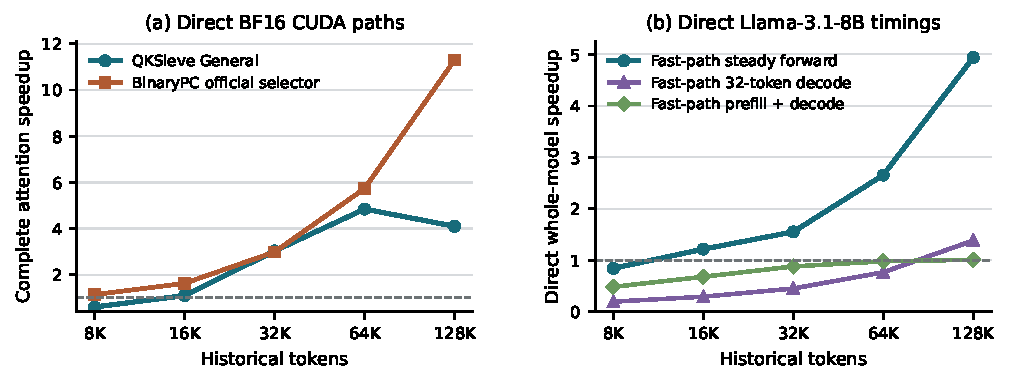
\includegraphics[width=\linewidth]{figures/qksieve_system_diagnostics.pdf}
  \caption{Direct RTX~3090 measurements.  Left: complete BF16 single-layer
  attention calls for General and the released BinaryPC selector.  Right:
  Fast-path Llama-3.1-8B steady forwards, measured 32-token decode intervals,
  and prefill-plus-decode requests; the right panel is a crossover diagnostic,
  not a General-profile speed claim.  No curve is reconstructed from a sum of
  independently timed stages.}
  \label{fig:speed}
\end{figure}

\begin{table}[!htbp]
\caption{Frozen native-MHA FP16 component timings on RTX~3090.  Components
are invoked independently to locate bottlenecks and are not summed to
reconstruct the directly timed complete path.}
\label{tab:deployment-breakdown}
\centering
\begin{tabular}{rrrrr}
\toprule
Length & Query prepare & Selector scan & Sparse attention & Complete path \\
\midrule
8K & .0336 & .0365 & .0438 & .1386 \\
16K & .0335 & .0468 & .0910 & .1946 \\
32K & .0299 & .0634 & .1107 & .2312 \\
64K & .0302 & .0999 & .1186 & .2684 \\
128K & .0303 & .1673 & .1630 & .3810 \\
\bottomrule
\end{tabular}
\end{table}

Query preparation is nearly length-independent.  The packed scan and exact
sparse consumer dominate at 128K, while candidate materialization, gather,
and launch overhead explain the gap between the independent stages and the
complete call.  Capping quantile samples at 512 specifically reduces the
long-context selector term; it does not change the linear packed-index scan.

\begin{table}[!htbp]
\caption{Earlier GQA-4 BF16 QKSieve Fast--Robust timing on RTX~3090.  Complete paths
are timed directly; scan and consumer rows are independently invoked
diagnostics and are not added.  Robust uses rank-16 block-affine INT4 Value
coefficients and $\alpha=.5$.}
\label{tab:robust-direct-timing}
\centering
\begin{tabular}{lrr}
\toprule
Direct operation, 128K & Time (ms) & Speed vs Full \\
\midrule
Full attention & 2.451 & 1.000$\times$ \\
Fast complete attention & .398 & 6.161$\times$ \\
Robust complete attention & .595 & 4.119$\times$ \\
General conditional complete call & .598 & 4.100$\times$ \\
Robust Key+Value-tail scan & .347 & -- \\
Robust exact-selected-plus-tail consumer & .190 & -- \\
\bottomrule
\end{tabular}
\end{table}

The Robust per-token index contains 240 Key bits, 64 Value coefficient bits,
and two amortized block-metadata bits, totaling 7.471\% of FP16 K+V.  Its
12-case whole-model geometric-mean steady speedup is 3.224$\times$; one-time
initialization amortized over 64 measured decode tokens gives 1.125$\times$.
These values are lower than Fast but pair with the independently validated
native-128K robustness result.

\begin{table}[!htbp]
\caption{Long-history physical CUDA attention scaling with a fixed
1,280-token exact-attention budget.  The 256K/512K rows sum 36 Qwen3-style
layers and exclude non-attention model work and first index construction.
The strict 256K diagnostic rejects this budget as quality-valid, and
Qwen3-4B does not natively support 512K quality; these rows therefore isolate
low-budget operator scaling.}
\label{tab:long-history-attention}
\centering
\begin{tabular}{lrrr}
\toprule
History & Full SDPA & \method & Speedup \\
\midrule
128K, one layer & 2.439 ms & .360 ms & 6.78$\times$ \\
256K, $B=1280$ & 175.008 ms & 12.650 ms & 13.83$\times$ \\
512K, $B=1280$ & 380.282 ms & 17.513 ms & 21.71$\times$ \\
\bottomrule
\end{tabular}
\end{table}

\begin{table}[!htbp]
\caption{High-fidelity long-history attention timing on one RTX~3090.
\method uses 24\% active tokens and includes Query projection/quantization,
low-bit retrieval, sampled-quantile selection, and exact sparse attention.
The pre-expanded baseline excludes GQA replication, whereas the HF-style
baseline includes \texttt{repeat\_kv} and SDPA.  Times sum 36 Qwen3-style
layers and exclude index construction and non-attention model work.}
\label{tab:long-history-highfidelity-attention}
\centering
\small
\resizebox{\linewidth}{!}{%
\begin{tabular}{lrrrrr}
\toprule
History & Pre-expanded SDPA & HF GQA+SDPA & \method & vs.\ pre-expanded &
vs.\ HF \\
\midrule
256K & 175.104 ms & 567.610 ms & 199.992 ms & .876$\times$ &
2.838$\times$ \\
512K & 348.520 ms & 1135.721 ms & 373.800 ms & .932$\times$ &
3.038$\times$ \\
\bottomrule
\end{tabular}}
\end{table}

Thus the high-fidelity sparse path is not faster than an idealized SDPA
consumer whose GQA K/V have already been materialized.  Its practical
advantage is relative to the actual HF execution path that performs GQA
replication at every decode step.  We report both denominators rather than
folding replication into an unspecified ``attention overhead.''  At 512K,
the 24\% selector uses 768 stratified samples ($c=128$) so that its confidence
capacity remains within the 16-way ragged-kernel limit.

An old 262,144-token-history plus 16-target stress test gives
Full/\method PPL 5.7518/5.1052 and 100\% top-1 agreement, but those target
positions exceed the declared model limit and are not a native-context
quality claim.  The registered native-boundary rerun instead uses 262,080
history plus 64 targets.  A 524,256-token Full prefill does complete on seven
RTX~3090 GPUs with 22.70 GiB peak allocated and 24.00 GiB peak reserved on
the busiest device.  However, Qwen3-4B has neither native positions nor RoPE
scaling beyond 262,144 tokens, and its extrapolated Full PPL on the diagnostic
window is 5510.6.  We therefore use 512K only to measure relative
Full--sparse approximation and system stress, not native task quality.

\begin{table}[!htbp]
\caption{Strict native-boundary 256K causal-PPL frontier over four
independently shuffled 20-Newsgroups windows (262,080 history plus 64 targets
per window; 256 paired target tokens).  Retention is computed from pooled
NLL differences.  The interval bootstraps the four windows as clusters and
is therefore diagnostic rather than a final cross-corpus confidence claim.}
\label{tab:256k-frontier}
\centering
\small
\resizebox{\linewidth}{!}{%
\begin{tabular}{rrrrr@{\qquad}r}
\toprule
Active & Retention (95\% CI) & Top-1 & KL & Steady & Online \\
\midrule
7.977\% & 94.440\% [93.38, 95.68] & 78.516\% & .04365 &
5.511$\times$ & 4.925$\times$ \\
9.977\% & 96.260\% [94.53, 97.73] & 82.031\% & .03266 &
5.345$\times$ & 5.097$\times$ \\
11.927\% & 96.949\% [94.79, 98.43] & 83.984\% & .02696 &
4.453$\times$ & 4.283$\times$ \\
15.951\% & 97.418\% [95.43, 99.07] & 83.594\% & .02250 &
3.642$\times$ & 3.377$\times$ \\
20.055\% & 99.072\% [97.62, 100.55] & 84.766\% & .01349 &
2.959$\times$ & 2.887$\times$ \\
\textbf{23.958\%} & \textbf{100.250\% [99.40, 101.06]} &
\textbf{92.188\%} & \textbf{.00733} & \textbf{2.989$\times$} &
\textbf{2.911$\times$} \\
\bottomrule
\end{tabular}}
\end{table}

The 23.958\% point statistically matches Full on these windows; retention
slightly above 100\% is not evidence that sparse attention generally improves
the model.  Averaged over the four runs, Full and \method steady decode are
588.942 and 197.019 ms/token, respectively.  Common prefill is 1058.826 s,
so request-level speedup reaches $2\times$ only after approximately 5,436
generated tokens.  The complete FP16 K/V remain GPU-resident: ``Active''
denotes exact-attention compute, not cache-memory retention.

\begin{table}[!htbp]
\caption{Strict-256K oracle budget diagnosis on the same four windows and
256 paired target tokens as \cref{tab:256k-frontier}.  Exact-QK computes
all historical FP16 QK scores before selecting the stated budget; the
low-bit proxy uses the frozen QK-balanced/Key-MSE 240-bit index and complete
proxy top-$k$.  Both consumers use exact attention over original FP16 K/V.}
\label{tab:256k-oracle-gap}
\centering
\small
\resizebox{\linewidth}{!}{%
\begin{tabular}{lrrrrrr}
\toprule
Selector & Exact/head & Active & Oracle mass & Retention (95\% CI) & Top-1 & KL \\
\midrule
Exact FP16 QK & 1,280 & .488\% & 90.002\% &
\textbf{100.240\% [99.48, 100.88]} & 90.625\% & \textbf{.00516} \\
Exact FP16 QK & 2,560 & .977\% & 93.057\% &
\textbf{100.148\% [99.54, 100.68]} & 92.969\% & \textbf{.00297} \\
Low-bit proxy & 1,280 & .488\% & -- &
80.771\% [77.84, 83.92] & 67.188\% & .24246 \\
Low-bit proxy & 2,560 & .977\% & -- &
86.132\% [84.68, 87.77] & 71.094\% & .15092 \\
\bottomrule
\end{tabular}}
\end{table}

\begin{table}[!htbp]
\caption{Matched 128K--256K selector crossover.  Both lengths use the same
frozen QK-balanced/Key-MSE template, complete proxy top-$k$, four text
windows and seeds, and 256 paired targets.  Entries are PPL retention with
four-window cluster-bootstrap 95\% intervals.}
\label{tab:128k-256k-selector-crossover}
\centering
\small
\resizebox{\linewidth}{!}{%
\begin{tabular}{lrrrr}
\toprule
History & Exact-1,280 & Proxy-1,280 & Exact-2,560 & Proxy-2,560 \\
\midrule
128K & 100.805\% [99.40, 102.23] & 98.993\% [96.53, 102.99] &
100.345\% [99.14, 101.57] & 100.005\% [97.66, 103.02] \\
256K & 100.240\% [99.48, 100.88] & 80.771\% [77.84, 83.92] &
100.148\% [99.54, 100.68] & 86.132\% [84.68, 87.77] \\
\bottomrule
\end{tabular}}
\end{table}

\begin{table}[!htbp]
\caption{Strict-256K coordinate--allocation split at top-1,280.  All rows
use the same four windows, 256 paired targets, complete top-$k$, and exact
attention over original FP16 K/V.  Online decode amortizes one-time selector
preparation over approximately 63 timed steps and excludes common prefill.}
\label{tab:256k-selector-cause}
\centering
\small
\resizebox{\linewidth}{!}{%
\begin{tabular}{lrrrrr}
\toprule
Selector/index policy & Retention (95\% CI) & Top-1 & KL & Steady & Online \\
\midrule
Exact FP16 QK & 100.240\% [99.48, 100.88] & 90.625\% & .00516 & -- & -- \\
Frozen coord./frozen bits & 80.771\% [77.84, 83.92] & 67.188\% & .24246 &
7.785$\times$ & 6.668$\times$ \\
Frozen coord./local bits & 89.911\% [84.13, 94.28] & 77.344\% & .13332 &
7.766$\times$ & 5.259$\times$ \\
Local coord./fixed bits & \textbf{100.443\% [99.80, 101.02]} & 91.016\% &
.00620 & 7.671$\times$ & \textbf{4.955$\times$} \\
Local coord./local bits & 100.430\% [99.78, 100.99] & 91.016\% &
.00622 & \textbf{7.733$\times$} & 4.055$\times$ \\
Frozen all-INT8 & 100.267\% [99.48, 100.91] & 91.016\% & \textbf{.00508} &
1.882$\times$ & 1.846$\times$ \\
\bottomrule
\end{tabular}}
\end{table}

\begin{figure}[!htbp]
\centering
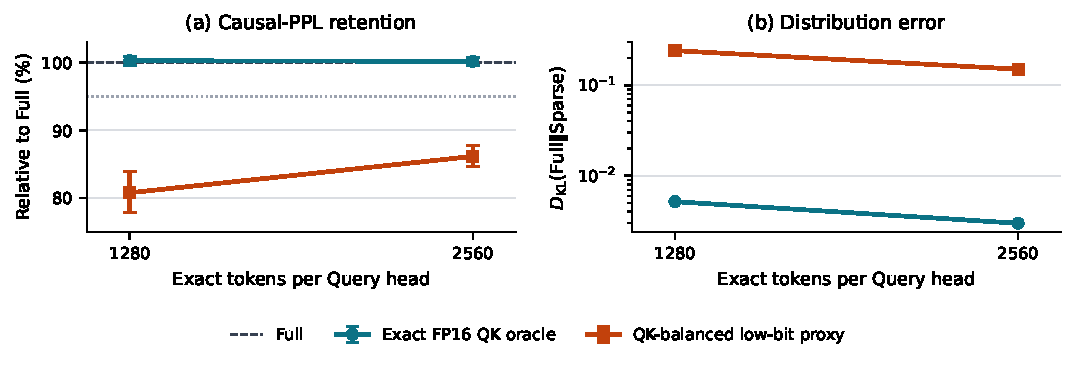
\includegraphics[width=.78\linewidth]{figures/qksieve_256k_oracle_gap.pdf}
\caption{At the native 256K boundary, 1,280 exact tokens per Query head are
already sufficient when selected by Exact FP16 QK.  Doubling the low-bit
proxy budget improves quality but leaves a large selection gap.  Error bars
are four-window cluster-bootstrap 95\% intervals.}
\label{fig:256k-oracle-gap}
\end{figure}

This control reverses the initial fixed-budget diagnosis.  Exact-QK
top-1,280 retains 100.24\% PPL with KL .0052 at only .488\% active, whereas
the frozen low-bit proxy retains 80.77\%; proxy top-2,560 reaches 86.13\%.
Under the matched 128K protocol, the same proxy retains 98.99\% and
100.01\%, respectively (\cref{tab:128k-256k-selector-crossover}).
Thus the 23.958\% point in \cref{tab:256k-frontier} compensates proxy
misranking rather than a fundamental attention budget.  The orthogonal split
in \cref{tab:256k-selector-cause} localizes the cause.  Reallocating the same
240 bits under frozen coordinates recovers only 89.91\%, whereas local
coordinates with fixed 4-1-1-1-1-1-0-0 bits recover 100.44\%, statistically
matching local coordinates plus local allocation (100.43\%).  Coordinate
shift is therefore dominant in this stress test; dynamic bits are neither
necessary nor measurably beneficial here.  Local fixed bits retain
7.67$\times$ steady and 4.96$\times$ 64-token online whole-model speed,
while frozen all-INT8 confirms that more precision can mask stale
coordinates at much lower speed.  We omit oracle speed because its dense
FP16 QK scan is diagnostic, not deployable.

\begin{table}[!htbp]
\caption{Qwen3-4B 512K extrapolation stress on one 20-Newsgroups causal-PPL
window (524,256 history plus 32 targets).  The absolute Full PPL is 5510.6;
retention therefore measures only proximity to the same extrapolated Full
distribution.  Online decode amortizes selector setup over the 31 timed
steps and excludes the common 4,297--4,299 s prefill.}
\label{tab:512k-extrap-frontier}
\centering
\small
\begin{tabular}{rrrrrrr}
\toprule
Active & Retention & Top-1 & KL & Steady & Online & Count range \\
\midrule
2.951\% & 105.34\% & 93.75\% & .0978 & 10.70$\times$ & 9.00$\times$ &
5,117--33,365 \\
3.947\% & 101.63\% & 96.88\% & .0794 & 10.72$\times$ & 8.13$\times$ &
6,999--48,828 \\
4.880\% & 99.97\% & 93.75\% & .0754 & 8.98$\times$ & 7.82$\times$ &
8,805--49,759 \\
5.872\% & 98.57\% & 96.88\% & .0592 & 7.72$\times$ & 6.85$\times$ &
11,359--66,293 \\
\bottomrule
\end{tabular}
\end{table}

\begin{table}[!htbp]
\caption{Matched LongBench selector screening on 160 strict Llama-3.1-8B
pairs (10 examples per task).  Every sparse row uses the same active-token
schedule and original-KV consumer.  FIER, Quest, RaBitQ, and SparQ rows are
audited formula/reference controls, not official optimized-system timings.}
\label{tab:baseline-placeholder}
\centering
\small
\begin{tabular}{lrrr}
\toprule
Method & Index bits/token/KV-head & Active & Full-relative quality \\
\midrule
Full & 0 & 100.00\% & 100.000\% \\
\method reference & 240 & 7.440\% & 99.789\% \\
FIER RTN-1 g32 reference & 256 & 7.440\% & 100.010\% \\
Quest-P16, page-rounded & 256 & 7.562\% & 92.217\% \\
RaBitQ RTN-1 reference & 224 & 7.440\% & 100.012\% \\
SparQ-R32 selector only & 0 & 7.440\% & 99.623\% \\
SparQ-R32 complete formula & 0 & 7.440\% & 99.950\% \\
UNIQUE-P8 equation reference & 258 & 7.494\% & 93.193\% \\
\bottomrule
\end{tabular}
\end{table}

\begin{table}[!htbp]
\caption{Released BinaryPC comparison.  Quality uses 160 strict LongBench
pairs (ten examples per task) and remains too small for a superiority claim.
Speed uses direct BF16 single-layer CUDA calls at 128K with the same $B(N)$
and exact sparse consumer; \method speed is its deployment selector, whereas
quality is its deterministic reference selector.}
\label{tab:binarypc-public-comparison}
\centering
\begin{tabular}{lrrrr}
\toprule
Method & Index bits & Active & Full-relative quality & 128K attention \\
\midrule
Full & 0 & 100.00\% & 100.000\% & 1.000$\times$ \\
BinaryPC released & 64 & 7.440\% & 99.250\% & 11.295$\times$ \\
\method & 240 & 7.440\% & 99.789\% & 6.798$\times$ \\
\bottomrule
\end{tabular}
\end{table}

The FIER row is a strict same-sample, same-budget reference-quality run; its
quality harness is not used for latency.  The Quest-P16 control stores
per-page extrema and loads complete 16-token pages.  The SparQ complete
formula adds its $r=32$ temperature, local window,
approximate selected mass, and running mean-Value correction.  The official
RaBitQCache efficiency artifact requires CUDA~12.8 and a modified vLLM; this
RTX~3090 environment uses an older PyTorch CUDA runtime, so we do not report a
fabricated native RaBitQ speed.  The current public Microsoft repository
provides RetroInfer, not a runnable artifact of original RetrievalAttention.
